\documentclass[exercice]{thedocument}%
\usepackage{texmaths-tikz}%
\startdatakeys
\source{}
\cycle{}
\competencesDuSocle{}
\connaissancesRequises{}
\competencesTravaillees{}
\enddatakeys
\begin{document}%
Reproduire la figure suivante en vraie grandeur.\par\centering
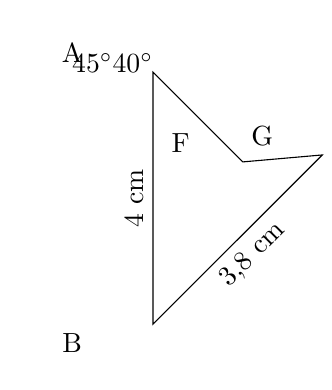
\begin{tikzpicture}[scale=0.8]
    \coordinate[label=above:A](A)at(0,0);
    \coordinate[label=below:B](B)at(0,-4);
    \path(A)--(B)([turn]135:3.8)coordinate[label=above right:G](G);
    \path(B)--(A)([turn]45:1)coordinate(F1);
    \path(B)--(G)([turn]-40:1)coordinate(F2);
    \coordinate[label=above right:F](F)at(intersection of A--F1 and G--F2);
    \tkzFillAngle[fill=Rainbow1-orange,size=0.6](B,A,F)
    \tkzMarkAngle[Rainbow1-orange!50!black,size=0.6](B,A,F)
    \tkzFillAngle[fill=Rainbow1-orange,size=0.6](G,B,A)
    \tkzMarkAngle[Rainbow1-orange!50!black,size=0.6](G,B,A)
    \tkzLabelAngle[Rainbow1-orange!50!black,pos=1](G,B,A){$45^\circ$}
    \tkzFillAngle[fill=Rainbow1-violet,size=0.6](F,G,B)
    \tkzMarkAngle[Rainbow1-violet!50!black,size=0.6,mark=none](F,G,B)
    \tkzLabelAngle[Rainbow1-violet!50!black,pos=1](F,G,B){$40^\circ$}
    \path(B)--(A)node[above,sloped,pos=0.5]{4 cm};
    \path(B)--(G)node[below,sloped,pos=0.5]{3,8 cm};
    \draw(A)--(B)--(G)--(F)--cycle;
\end{tikzpicture}
\end{document}
